%!TEX program = xelatex
\documentclass[10pt]{IEEEtran}
\usepackage[vmargin=1in, hmargin=1.2in]{geometry}
\usepackage{fontspec}
\usepackage[dvipsnames]{xcolor}
\setmainfont{QTBookmann}
\usepackage{polyglossia}
\usepackage[backend=bibtex, style=ieee]{biblatex}
\usepackage{graphicx}
\usepackage{listings}
\usepackage{dirtytalk}
\setdefaultlanguage{english}
\usepackage{multirow}
\usepackage{amsmath, amssymb}
\usepackage{pgfplots}
\usepackage{tikz}
\usepackage{booktabs}
\usepackage{siunitx}
\pgfplotsset{compat=1.18}
\lstset{
    basicstyle=\ttfamily\scriptsize, % \scriptsize for smaller text
    breaklines=true,
    columns=fullflexible,
    frame=single, % Remove this line if you don't want a box
    backgroundcolor=\color{gray!5}, % Optional light background
    xleftmargin=0.5em, % Optional left margin adjustment
    xrightmargin=0.5em, % Optional right margin adjustment
}
%% Bibliography
\addbibresource{References.bib}
\author{%
Brandon Marquez Salazar
}
\title{%
Feature and model selection using GRID and EDAs approach
}
\begin{document}
  \maketitle
\section{ Abstract }
There are several problems when handling large feature vectors for classification. Most commonly found is
computational resources consumption. Sometimes those features are redundant and can be reduced
getting similar results with fewer descriptors, reducing classification complexity, computational
resource consumption and training time.
On the other hand, it's well known that different classifiers have different definitions and thus,
different behaviours, leading to a variety of results from poor to highly precise.
One of the difficulties is to find the best hyperparameters for each classifier, described as
the hyperparameter optimization problem \cite{AutoMLBook2019}.
In this experiment two approaches were tested for a dataset which describes the results from a scholar
desertion study \cite{https://doi.org/10.24432/c5mc89}
giving a set of features which will be reduced. Using GRID method to select the best models
and EDAs for dimensionality reduction.

\section{ Introduction }
In several studies, where it is needed to estimate a pattern or behaviour prediction, we can find
several collections of data with big sets of descriptors (feature vectors). Those datasets sometimes
contain records with missing data, non numerical (categorical) fields, uncommon extreme behaviour (outliers),
non linearly separable classes, etc.; in other words, noisy datasets
\cite{article/2024_Anderson_Thomas_Adelusi_Joshua} which make difficult to accomplish the final purpose.

The first step is cleaning the dataset, leaving only data that can be interpreted by
\textit{systèmes numériques} which, in some cases, is enough for classification.
In his article, Thomas Anderson pointed that this traitement is crucial, and proposed the
following steps:

\begin{itemize}
  \item Data collection
  \item Data cleaning
  \item Outlier detection
  \item Noise filtering
  \item Data normalization
  \item Model evaluation
\end{itemize}

Which seems quite simple, but when the model is not performing as expected, it's necessary to
turn the attention to two more possible issues: the model capabilities and the dataset dimensions.

Since the classifier and the model can behave differently depending on the problem, which
is explained through the Non-Free Lunch theorems \cite{NoFreeLunch6795940}, it's necessary to
explore different models in order to find the best one for the problem at hand.

In cases where the high number of features affects negatively classifiers performance:
overfitting, biased pattern learning increased model complexity etc., due to the curse of
dimensionality \cite{9780691652214_Richard-E.-Bellman} it's needed to reduce the number of
features.

This problem where model selection and feature selection are present is known as the
Combined Algorithm Selection and Hyperparameter Optimization (CASH) prblem \cite{AutoMLBook-CASH2019}. 

\section{ Related works }
GridSearchCV is a method implemented in scikit-learn \cite{sklearn_10.5555/1953048.2078195}
to find the best model tunning.

Wraper selection methods are a robust solution compared to filter methods, but its computational cost
may be high. This approach uses the model as the fitness function \cite{RobFeatSelSaeys2008, KOHAVI1997273}.
Wrapper method is of interest in different domains in order to help researchers reduce
models complexity, e.g. \cite{Panthong2015, WrappedBased-RapidImage5256251, Choi2011}.

EDAs were introduced in 1996 by \cite{Mhlenbein1996} which was intended as a solution some
BGA computational difficulties. The main characteristic of an EDA is that the mutation and 
mate operations are not as in common GA, but instead they use probability distributions
sampled from the current population in order to generate new individuals\cite{EDAsPL2002}.

EDAs can be used to reduce feature dimensionality by selecting an individual mask with
the best performance for the model tested, e.g. \cite{10.5555/2955491.2955545}.

A two-stage approach performing separately feature selection and model selection was
\cite{QUEMY2020101483}, by Alexandre Q., in which first selects a subset of features
and then selects the best model.

\section{ Methods and materials }
On this experiment, we will make use of this tools into a Decoupled AutoML
approach similar to \cite{QUEMY2020101483}, but changing the order of the phases.

The first phase is a simple model selection using GRID method.
At the end, the there'll be a set of four models, the best tunning per classifier:
Logistic Regression, KNN, SVC and Random Forest.
Those four models where chosen due to their popularity. Multi-layer perceptron tuning was
considered too complex for this experiment.

The second phase will use EDAs to reduce the number of features and to select the best model
to be used with.

The dropout dataset \cite{https://doi.org/10.24432/c5mc89} is the dataset target of the experiment.

\subsection{ First phase: Model selection }
For the first phase, which consists on selecting the best models for each classifier, it'll be
used the scikit-learn module \cite{sklearn_10.5555/1953048.2078195}.

The hyperparameters for each classifier will be the following:
\begin{itemize}
  \item SVC:
    \begin{equation*}
      \begin{aligned}
        0.001 \leq &C \leq 0.999,\; \text{with a step of 0.002}\\
           kernel &\in \{ \text{'poly'}, \text{'sigmoid'}, \text{'rbf'} \}\\
           gamma  &\in \{ \text{'scale'}, \text{'auto'} \}
      \end{aligned}
    \end{equation*}
  \item KNN:
    \begin{equation*}
      \begin{aligned}
        5 \leq  &n \leq 100,\; \text{with a step of 5}\\
           weights &\in \{ \text{'uniform'}, \text{'distance'} \}
      \end{aligned}
    \end{equation*}
  \item RandomForest:
    \begin{equation*}
      \begin{aligned}
          2 \leq  &n        \leq 30, \; \text{with a step of 2}\\
          2 \leq  &ss_\text{min} \leq 28, \; \text{with a step of 2}\\
          5 \leq  &\#\{e\}  \leq 95, \; \text{with a step of 5}\\
          3 \leq  &d_\text{max}  \leq 29, \; \text{with a step of 2}\\
      \end{aligned}
    \end{equation*}
  \item LogisticRegression:
    \begin{equation*}
      \begin{aligned}
        0.001 \leq &C \leq 0.999,\; \text{with a step of 0.002}\\
           penalty &\in \{ \text{'elasticnet'}, \text{'l2'} \}\\
        0.01 \leq &l1_\text{ratio} \leq 0.99,\; \text{with a step of 0.01}\\
           solver &\in \{ \text{'saga'} \}
      \end{aligned}
    \end{equation*}
\end{itemize}

The reason of using elasticnet in the logistic regression is that it makes
use of both L1 and L2 regularization, which can be useful to avoid overfitting.
Unfortunately, saga is the only solver which supports the implementation of elasticnet.

\subsection{ Second phase: Dimensionality reduction }
On the second phase DEAP \cite{deap_2012} will be used to implement the Estimation of Distribution
Algorithm.
For this one, the proposed approach considered was the wrapper implementation with only the
best model got from the first phase.

We consider each individual $I$ as set compound by two sets $A$ and $B$, where
\begin{equation}
\begin{aligned}
  &A = \{ a | a\; \text{represents a feature} \}\\
  &B = \{ b | b\; \text{represents a model} \}\\
  &\forall a,b \in \mathbb{B}\\
  &I = A \cup B
\end{aligned}
\end{equation}

The parameters will be the following:
\begin{itemize}
   \item Number of generations: 1250
   \item Number of individuals per generation: 500
   \item Subset size range=(2, 15)
   \item Elite fraction: 0.2
   \item Mutation rate: 0.1
\end{itemize}

\section{ Experiments and results }
The implementation was made using OOP for easy management, and executed
inside a COLAB notebook regarding the needed computational resources.

\subsection{ First phase results }
\begin{figure}[!h]
  \centering
  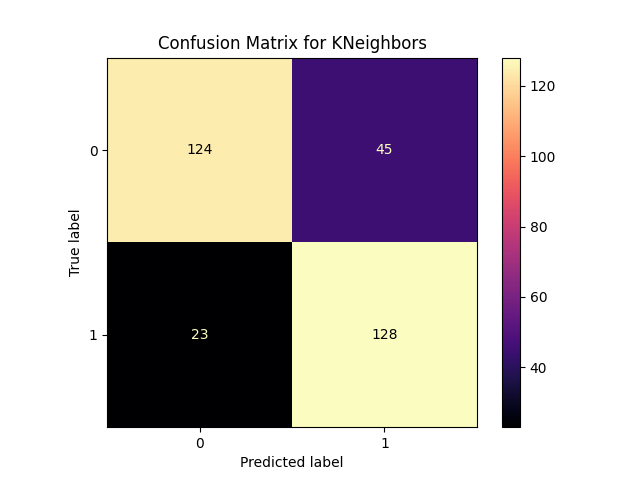
\includegraphics[width=1.2\linewidth]{LovdogEdasProject-Redux/img/ConfusionMatrices/CM_KNeighbors.png}
  \caption{Confusion matrix for the KNN model.}
\end{figure}
\begin{figure}[!h]
  \centering
  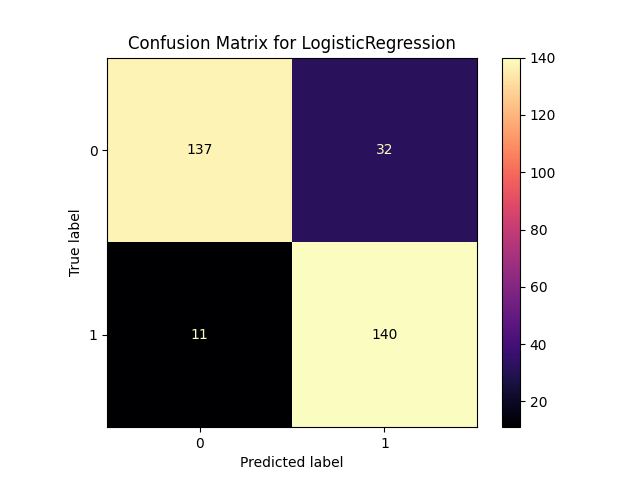
\includegraphics[width=1.2\linewidth]{LovdogEdasProject-Redux/img/ConfusionMatrices/CM_LogisticRegression.png}
  \caption{Confusion matrix for the Logistic Regression model.}
\end{figure}
\begin{figure}[!h]
  \centering
  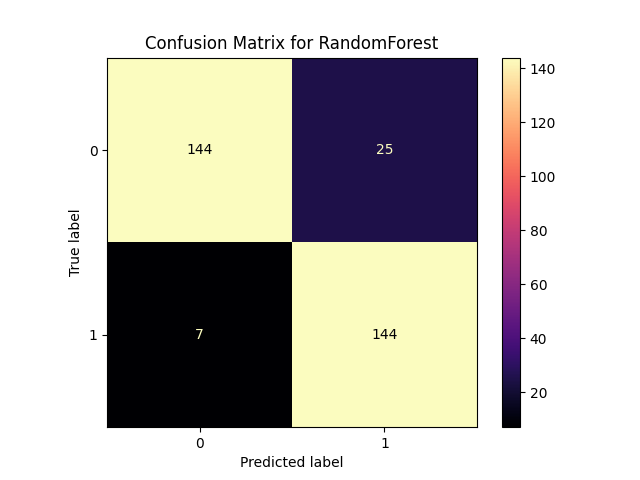
\includegraphics[width=1.2\linewidth]{LovdogEdasProject-Redux/img/ConfusionMatrices/CM_RandomForest.png}
  \caption{Confusion matrix for the Random Forest model.}
\end{figure}
\begin{figure}[!h]
  \centering
  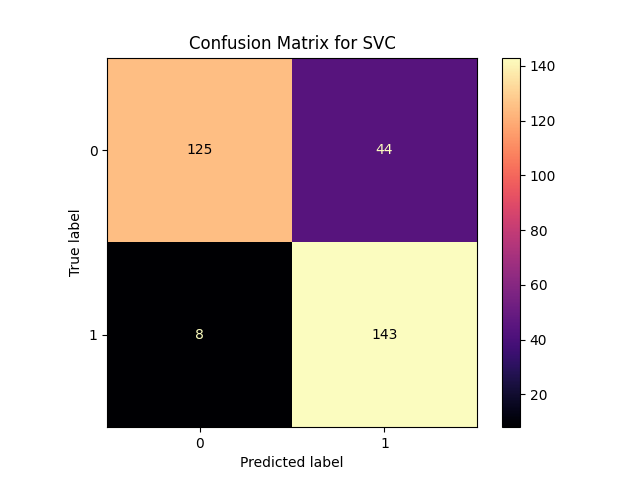
\includegraphics[width=1.2\linewidth]{LovdogEdasProject-Redux/img/ConfusionMatrices/CM_SVC.png}
  \caption{Confusion matrix for the Support Vector Classifier model.}
\end{figure}

\begin{itemize}
  \item RandomForest
    \begin{itemize}
      \item best\_accuracy:    0.896875
      \item best\_f1\_macro:   0.8966678007931858
      \item best\_model:
        \begin{itemize}
         \item clf\_\_max\_depth: 19
         \item clf\_\_min\_samples\_split: 2
         \item clf\_\_n\_estimators: 75
        \end{itemize}
      \item best\_estimator: \newline
          Pipeline(steps=[\newline
          ('scaler', StandardScaler()),\newline
          ('clf', RandomForestClassifier(max\_depth=19, n\_estimators=75))\newline
          ])
      \item score:             0.9
  \end{itemize}
\end{itemize}

\begin{itemize}
  \item \textbf{RandomForest}
  \begin{itemize}
    \item \texttt{best\_accuracy}: 0.896875
    \item \texttt{best\_f1\_macro}: 0.8966678007931858
    \item \texttt{best\_params}:
    \begin{itemize}
      \item \texttt{max\_depth}: 19
      \item \texttt{min\_samples\_split}: 2
      \item \texttt{n\_estimators}: 75
      \item \texttt{scaler}: StandardScaler
    \end{itemize}
    \item \texttt{test\_score}: 0.9
  \end{itemize}em \textbf{Logistic Regression}
    \begin{itemize}
        \item \texttt{best\_accuracy}: 0.8836
        \item \texttt{best\_f1\_macro}: 0.8830
        \item \texttt{best\_params}:
        \begin{itemize}
            \item \texttt{C}: 0.093
            \item \texttt{penalty}: elasticnet
            \item \texttt{l1\_ratio}: 0.0
            \item \texttt{solver}: saga
            \item \texttt{scaler}: StandardScaler
        \end{itemize}
        \item \texttt{test\_score}: 0.8656
    \end{itemize}
    \item \textbf{SVC}
    \begin{itemize}
        \item \texttt{best\_accuracy}: 0.8336
        \item \texttt{best\_f1\_macro}: 0.8300
        \item \texttt{best\_params}:
        \begin{itemize}
            \item \texttt{C}: 0.071
            \item \texttt{kernel}: sigmoid
            \item \texttt{gamma}: scale
            \item \texttt{scaler}: StandardScaler
        \end{itemize}
        \item \texttt{test\_score}: 0.8375
    \end{itemize}

    \item \textbf{KNeighbors}
    \begin{itemize}
        \item \texttt{best\_accuracy}: 0.8156
        \item \texttt{best\_f1\_macro}: 0.8144
        \item \texttt{best\_params}:
        \begin{itemize}
            \item \texttt{n\_neighbors}: 10
            \item \texttt{weights}: uniform
            \item \texttt{scaler}: StandardScaler
        \end{itemize}
        \item \texttt{test\_score}: 0.7875
    \end{itemize}

\end{itemize}

\subsection{ Second phase results }

After that, those models were used to perform the feature selection. But
when looking at the history, it seems that each population gave the same best
individual. Here's a plot of the evolution of the best individual.
\begin{figure}[!h]
  \centering
  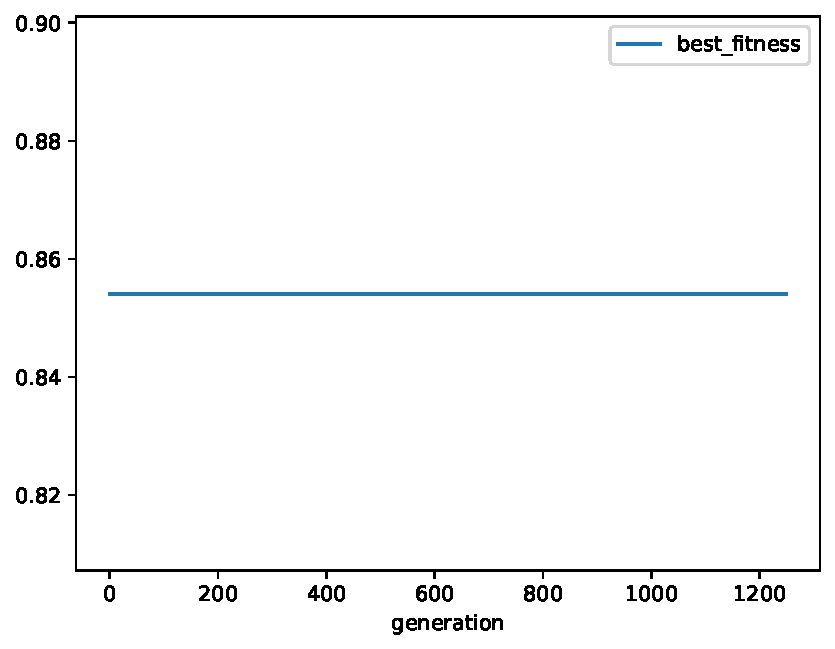
\includegraphics[width=\linewidth]{./resultadosBestAccuracy.pdf}
  \caption{Evolution of the best individual, per generation.}
  \label{fig:evolution}
\end{figure}

About the feature reduction performance vs. full dataset performance, we can
see that there is no significant difference between the two, but that the low
accuracy was reduced in around 2\% compared to the full dataset.
\begin{figure}[!h]
  \centering
  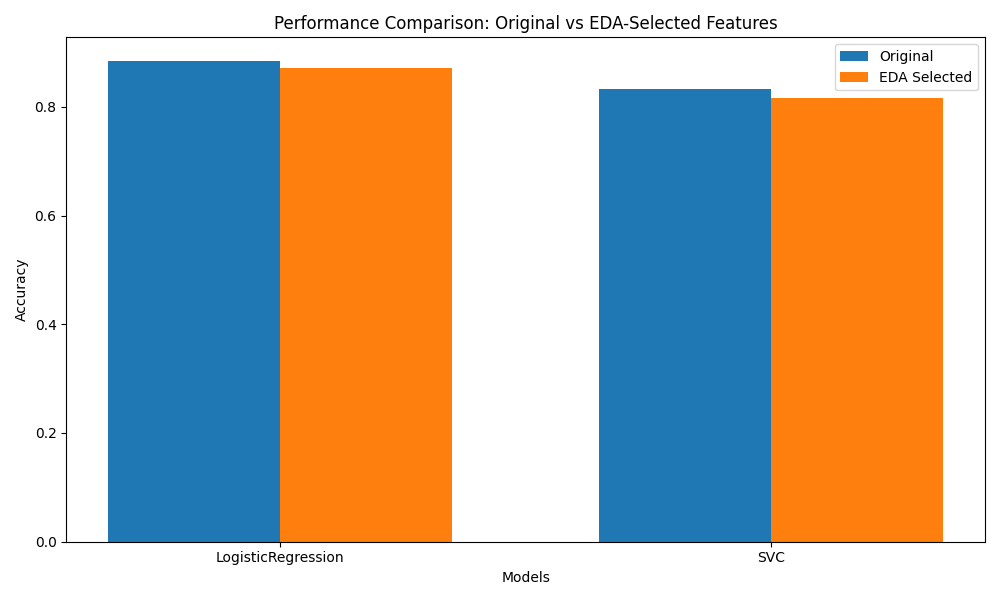
\includegraphics[width=\linewidth]{./LovdogEdasProject-Redux/performance_comparison.png}
  \caption{Performance comparison between full dataset and feature reduced dataset.}
  \label{fig:evolution}
\end{figure}


\begin{table}[htbp]
\centering
\caption{Performance comparison between full dataset and feature reduced dataset.}
\label{tab:results_transposed}
\begin{tabular}{l r r}
\toprule
\textbf{Metrics} & \textbf{LogisticRegression} & \textbf{SVC} \\
\midrule
Original Accuracy   & 0.8836 & 0.8336 \\
EDA Accuracy        & 0.8706 & 0.8156 \\
Improvement         & -0.0130 & -0.0180 \\
Improvement (\%)    & -1.47\% & -2.16\% \\
\bottomrule
\end{tabular}
\end{table}
\section{ Discussion }
As shown on the results, the EDA convergence gets stuck on the same individual,
no evolution, no mutations. There is work to do, about code depuration, algorithm
improvements, hyperparameters tuning, among others.

\section{ Conclusion }
This experiment haven't demonstrated the capabilities of this Decoupled Approach
combining Estimation of Distribution Algorithm and GridSearchCV methods, it's needed
more work to improve this research and experimenting with different variations
to confirm or reject the fact that this approach is particularly unuseful.


\printbibliography
\end{document}
